%************************************************
\chapter{Descripción de compresión JPEG con pérdida}\label{ch:jpeg_desc}
%************************************************

\section{Introducción Breve de Términos Matemáticos}

A continuación se dan introducciones breves a conceptos que serán utilizados y
explicados a mayor detalle en el capítulo \ref{ch:implementacion}

El nacimiento de la Teoría de la Información en 1948 marcó el inicio del
estudio formal de la compresión de datos. Surgió con la publicación del
artículo de Claude E.  Shannon ``A Mathematical Theory of Communication''
\cite{shannon}, donde se introdujeron los conceptos de \emph{densidad},
\emph{entropía} y \emph{redundancia} de información.

% La Codificación de Entropía son métodos de \gls{compresión sin pérdida} de
% información que no toman en cuenta el contenido. Los dos métodos más populares
% actualmente son los Códigos de Huffman y la Codificación Aritmética.

Dos años después de la publicación de Shannon, David Huffman inventó lo que hoy
conocemos como codificación huffman \cite{Huffman}. Los \gls{códigos de Huffman} son
códigos de prefijos que minimizan la longitud de los códigos individuales. Se
mantienen hasta hoy como la técnica más aprovechada en algoritmos de compresión
sin pérdida.

Después de Huffman, el método más popular para reducir redundancia es la
\gls{codificación aritmética}. Es un método más sofisticado que consigue
mejores resultados. Entre $5\%$ y $10\%$ según el estándar JPEG
\cite{jpeg-spec}. La especificación de la compresión JPEG incluye la capacidad
de utilizar codificación aritmética, pero en la práctica tiende a no ser usada.
Las razones tienen que ver con el alto número de patentes relacionados a la
codificación aritmética. \cite{jpeg_patents}.

En 1974, Nasir Ahmed publicó un artículo describiendo su transformada de coseno
discreta (\emph{DCT}, por sus siglas en inglés) \cite{ahmed_dct}. La \gls{DCT} es un
caso particular de la transformada de Fourier, restringida a los números
reales.

La compresión JPEG, como usualmente se usa, está basada en códigos de Huffman y en
la transformada de coseno discreta.

% ============================================================
\section{Tipos de compresión}
% ============================================================

La compresión de datos puede ser \emph{con pérdida} o \emph{sin pérdida}. Una
\gls{compresión sin pérdida} es una función biyectiva. El dominio de la función
es el espacio de datos que estamos interesados en comprimir. Los formatos de
compresión sin pérdida funcionan identificando información redundante y
removiendo la redundancia, dejando la información intacta. La compresión con
pérdida tiende a hacer lo mismo que la que no tiene pérdida, pero encima
identifica información que juzga como ``innecesaria''. Es decir, información
que puede ser descartada sin un cambio importante en la interpretación humana.

El formato JPEG soporta varios tipos de compresión.

\begin{list}{}{} \item \emph{Baseline}

El tipo \emph{\gls{baseline}} es el más popular y es el tipo de compresión en el que
se enfoca este trabajo. Por brevedad, a menos de que se especifique lo
contrario, cuando el resto de este documento hable de compresión JPEG, estará
hablando del tipo \emph{baseline}. La compresión está basada en la Transformada
de Coseno Discreta para filtrar información innecesaria, y para reducir
redundancia puede utilizar árboles de Huffman o codificación aritmética.

\item \emph{Progresivo}

El tipo \emph{progresivo} es similar a \emph{baseline}, pero se le agregan
propiedades deseables. La imagen se comprime en múltiples pasos, cada uno con
mayor detalle. Con el método \emph{progresivo}, se puede desplegar la imagen
sin que se tenga la totalidad de los datos en memoria. Esto es útil para poder
dibujar la imagen mientras se está descargando de Internet. Cuando se está en
un entorno con ancho de banda limitado, o cuando se descarga una imagen muy
grande, es de valor para el usuario poder ver versiones de la imagen
progresivamente más detalladas mientras se descarga.

\item \emph{Sin pérdida}

Aunque el estándar JPEG incluye la posibilidad de compresión sin pérdida, el
artículo en el que se presenta JPEG \cite{jpeg-paper} hace notar que no hubo un
análisis riguroso para su diseño.

La compresión JPEG sin pérdida no es mala, pero formatos como PNG o TGA son más
populares y efectivos. Aunque está incluida en la especificación, mucho
software simplemente no soporta JPEG con compresión sin pérdida.

\item \emph{Compresión Jerárquica}

El modo jerárquico codifica la imagen en varias versiones, cada una a
diferentes resoluciones. Se guarda en una estructura ``piramidal''. La primera
imagen está comprimida a resolución completa, y cada imagen sucesiva se guarda
a la mitad de la resolución de la anterior.

Este método es útil cuando la resolución de la imagen es muy grande, y la
aplicación no necesita o no es capaz de utilizar la imagen en su tamaño
completo.

\end{list}

% ============================================================
\section{Descripción de la Compresión \emph{Baseline} de JPEG}
% ============================================================

El codificador implementado en este trabajo es el \emph{Baseline JPEG}, al que
también se le refiere como \emph{DCT-Based Coding}, traducido aquí como
\emph{Codificación DCT}. Para el resto del documento, a menos que sea
necesario, se usará el término \emph{JPEG} para referirse a lo mismo que
\emph{Baseline JPEG}.

La codificación DCT divide a la imagen en bloques de $8\times8$ píxeles. Cada
bloque de $8\times8$ pasa por una serie de transformaciones y salen
secuencialmente como datos comprimidos.

El primer paso en el \emph{pipeline} es separar los componentes de la imagen.
Las dos maneras más comunes de representar imágenes en computadoras es
\verb+RGB+ o \verb+RGBA+: En ambos formatos, cada píxel ocupa 32 bits de
espacio, divididos en componentes de 8 bits. Cada componente corresponde a un
color o al valor de opacidad, comúnmente denominado \emph{alfa}. \verb+RGB+
corresponde al byte \verb+RRGGBBXX+, con \verb+RR+ representando rojo,
\verb+GG+ representando verde y \verb+BB+ representando azul. Aunque a veces
decimos que \verb+RGB+ es un formato de 24 bits, especificamos el byte
\verb+XX+ por convención, ya que siempre se utilizan 32 bits (4 bytes) para
representar RGB. \verb+RGBA+ es análogo a \verb+RGB+. Le corresponden los 4
bytes \verb+RRGGBBAA+, donde el último byte se usa para el valor \emph{alfa}.

% \subsection{Endianness}

% % Nota para edicion: DWORD es usado por intel & MS. No introducir nuestra propia pinche notación...

% Cabe notar que diferentes plataformas tienen diferentes convenciones para
% guardar colores en memoria. Windows espera que le mandemos píxeles en órden
% \verb+BGRA+, ya que al inspeccionar la memoria se ve en el órden más familiar
% de \verb+ARGB+ (Microsoft no ha dicho públicamente por qué reordenaron los
% componentes de color pero no el de opacidad).

% Este tema toca el concepto de \emph{endianness}, que es el término que usamos
% para referirnos al orden de los bytes en una doble palabra de memoria. En
% procesadores modernos, una doble palabra son 32 bits. 4 bytes, cada uno de 8
% bits. Cuando nos importan los detalles de bajo nivel entonces debemos de
% entender la diferencia entre arquitecturas \emph{little endian} y \emph{big
% endian}. Una arquitectura \emph{Little endian} guarda los bytes en registros
% de izquierda a derecha del menos significativo al más significativo. Es más
% claro usar el ejemplo concreto de los colores representados en palabras de 32
% bits. Un color \verb+RGBA+ consiste de 4 bytes y en una máquina little endian
% se guarda en la memoria de la computadora como \verb+ABGR+. En una máquina
% \emph{big endian}, se representa de la misma manera en que se escribe:
% \verb+RGBA+. En ambos tipos de ordenamiento de memoria, su \emph{endianness}
% afecta solamente al ordenamiento de bytes dentro de registros de la máquina. No
% hay que confundirnos y pensar que el efecto se extiende más allá de lo que cabe
% en un registro. Si tenemos dos palabras \verb+U = abcd+ y \verb+V = efgh+
% entonces \verb+UV+ se ve en memoria como \verb+dcbahgfe+. Los bytes se voltean
% dentro de las palabras individuales, pero las palabras siempre van de izquierda
% a derecha. Procesadores ARM después de la versión 3 son \emph{bi-endian},
% pueden seleccionar su \emph{endianness} desde software. Los procesadores x86,
% hoy en día, son exclusivamente little endian.

% En ensamblador con sintaxis de Intel o en el API de Windows, se utiliza
% \verb+BYTE+ para denotar 8 bits, \verb+WORD+ para 16 bits, \verb+DWORD+ para 32
% bits y \verb+QWORD+ para 64 bits. Esta convención viene de cuando los
% procesadores eran de 16 bits, y no cambió ni en la transición a 32 bits en los
% 90's ni en la transición a 64 bits en los 00's

% El codificador JPEG que escribimos asume que la máquina en la que se está
% corriendo es \emph{little endian}.


\subsection{La DCT}

La transformada discreta de coseno puede representar $N$ puntos como una suma
con pesos de funciones cosenoidales de diferentes frecuencias. Es popular en
compresión porque las señales que comprimimos tienden a tener una
representación con bajas frecuencias predominantes. Por ejemplo, es más común
una imagen de un cielo azul que una que tiene ruido blanco. Una imagen de un
cielo azul tiene muy poca variación, que al aplicar \emph{DCT} resulta en un
peso alto para frecuencias bajas y pesos más cercanos a cero para frecuencias
más altas.

En JPEG se divide la imagen en bloques de $8\times8$ y se utiliza una
\emph{DCT} de $8\times8$:

\begin{equation}\label{eq:dct}
F(u, v) = \frac{1}{4} C(u)C(v) \sum_{x=0}^{7}\sum_{y=0}^{7}
f(x,y)*\cos{\frac{(2x+1)u\pi}{16}}\cos{\frac{(2y+1)v\pi}{16}}
\end{equation}

donde \[C(u), C(v) = \begin{cases}
        \frac{1}{\sqrt{2}} & \quad \text{para } u,v = 0\\
        1                  & \quad \text{para } u,v \neq 0\\
\end{cases} \]
\begin{eqnarray*}
    f(u, v) \text{ es un punto del bloque de } 8\times8 \text{ de la imagen }\\
    F(u, v) \text{ es la DCT para el punto } u,v\\
\end{eqnarray*}

De la ecuación \ref{eq:dct} se puede derivar directamente un algoritmo para la
\emph{DCT}, visto más a detalle en el capítulo \ref{ch:implementacion}.

La función $F$ definida en \ref{eq:dct} es una función continua e invertible, y
su inversa es:

\begin{equation}\label{eq:idct}
f(x, y) = \frac{1}{4} \sum_{x=0}^{7}\sum_{y=0}^{7} C(u)C(v) F(u, v)*
\cos{\frac{(2x+1)u\pi}{16}}\cos{\frac{(2y+1)v\pi}{16}}
\end{equation}

Nótese entonces que en teoría es posible convertir los puntos de cada bloque de
$8\times8$ a su forma en DCT y de regreso. La ventaja de tener cada bloque como
coeficientes DCT es que su representación nos permite decidir \emph{qué
información perder}.

\subsection{La vida de un bloque}\label{sub:vida}


JPEG trabaja dividiendo a la imagen en bloques cuadrados de 8 pixeles de ancho
y alto. Si el tamaño de la imagen no es un múltiplo de ocho, se redondea al
siguiente múltiplo de ocho. El decodificador hace lo mismo y sabe ignorar los
píxeles sobrantes.

Cada bloque pasa por varias etapas antes de ser escrito a memoria como bits
comprimidos de JPEG.


\subsection{YUV}\label{sub:yuv}

Cada bloque crudo de la imagen se convierte en tres nuevos bloques, cada uno
correspondiente a un componente del modelo de color \gls{YUV}, también
denominado \verb+YCbCr+

Un modelo de color es una manera abstracta de representar colores. \verb+RGB+
representa colores como combinaciones de tres colores primarios. \verb+YUV+ los
representa en tres componentes, uno para Luminancia y dos de Crominancia.

\gls{luminancia}, también llamado luma o \verb+Y+, es la intensidad de la imagen. La
\gls{crominancia}, también llamada chroma, describe el color de la imagen y se
codifica con dos componentes \verb+U+ o \verb+Cb+ y \verb+V+ o \verb+Cr+, donde
$U = Azul - Luminancia$ y $V = Rojo - Luminancia$.

El modelo de color \verb+YUV+ se inventó con la llegada de la televisión a
color. La luminancia no es otra cosa que la imagen en blanco y negro. La
transición al color se hizo gradualmente transmitiendo la información de la
misma manera que antes, pero usando dos nuevos canales, \verb+U+ y \verb+V+. De
esta manera, el nuevo formato era compatible con televisiones en blanco y
negro, que sólo necesitaban la información de uno de los canales.

\begin{figure}[hb]
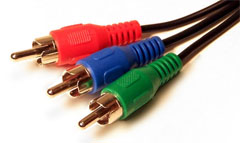
\includegraphics{yuv_cable}
    \caption{Cable YUV}
\end{figure}

Los cables RCA empezaron transmitiendo los tres componentes de \verb+YUV+. Más
tarde, cuando todos tenían color, se migró a usar un cable para \gls{YUV},
llamado video compuesto, dejando a los otros dos cables para sonido estéreo.

\begin{figure}
    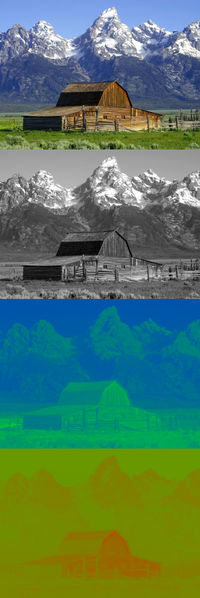
\includegraphics{yuv}
    \caption{Descomposición de una imagen a un canal de Luma y dos de Chroma}
\end{figure}

\verb+YUV+ tiene ventajas para comprimir imágenes. El sistema de visión humano
es mucho más sensible a cambios de intensidad en la imagen que a cambios de
color. Esto se aprovechaba en los días de la televisión analógica para utilizar
más ancho de banda en Luma que en Chroma, y el mismo principio se utiliza en
JPEG, cuya especificación incluye la opción de usar resoluciones más bajas para
los canales chroma que los luma.

% TO-DO: MOVER ESTE PARRAFO A IMPLEMENTACION
La implementación de \verb+tiny_jpeg+ usa la misma resolución para los tres canales.

Los tres bloques correspondientes a \verb+Y+, \verb+U+, y \verb+V+ son escritos
al archivo en ese orden después de ser transformados independientemente.

\subsection{Aplicación de DCT y Cuantificación}\label{sub:vida_dct}

\begin{figure}[h]
    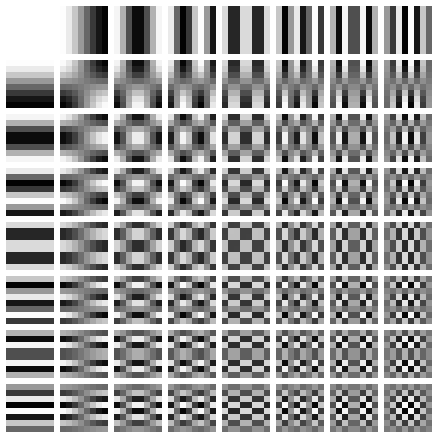
\includegraphics{DCT-8x8}
    \caption{Visualización de las funciones para el DCT de 8x8 usado en JPEG.
    Esquina superior izquierda: menor frecuencia. Inferior derecha: mayor
frecuencia.}
    \label{fig:dct}
\end{figure}



A cada bloque se le aplica la Transformada Discreta de Coseno de $8\times8$. El
resultado son 64 coeficientes para las 64 funciones base. Como se muestra en la
figura \ref{fig:dct}, la frecuencia se incrementa hacia la derecha y abajo. Por
eso a partir de este momento se itera el bloque en un patrón de zig-zag
\ref{fig:zigzag}, empezando en la esquina superior izquierda y acabando en la
inferior derecha.

\begin{figure}[h]
    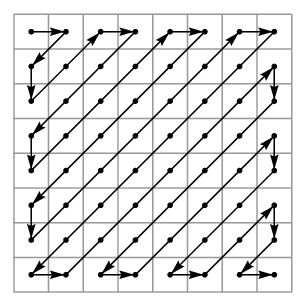
\includegraphics{zigzag}
    \caption{El patrón zig-zag con el que se itera por los bloques.}
    \label{fig:zigzag}
\end{figure}

En la descripción de la DCT se menciona que tener a cada bloque como
coeficientes DCT nos facilita la elección de qué información perder. En
principio, se pierde algo de información al aplicar la función DCT y luego su
inversa, sólo por el hecho de que estamos trabajando con una máquina con
precisión finita. Encima, el hecho de que JPEG especifica usar enteros de 10
bits o menos hace que se pierda un poco más información durante el proceso de
redondear valores de punto flotante. Aunque esos efectos de pérdida de
información no son negligibles, la principal manera en que se elige qué
información perder son las \gls{tablas de cuantificación}.

A cada codificador, usualmente elegido por heurísticas \emph{ a priori }, le
corresponden al menos dos tablas de cuantificación de 64 elementos. El propósito
de estas tablas es decidir cuánta información queremos perder para diferentes
coeficientes DCT. \emph{Cuantificación} es el proceso de convertir un conjunto
de valores a otro conjunto más pequeño. Para JPEG usamos división entera para
cuantificar los elementos de cada bloque. El concepto se puede explicar con un
ejemplo:

Supongamos que tenemos el conjunto de valores $ \{ 1, 5, 103, 128, 242 \} $ que
queremos cuantificar usando división entera: Todos los elementos $e_i$ se
reducen a $ n_i \text{ tal que } e_i = n_i * c + r \text{ con } n \in ℕ \text{
y } c \text{ la constante de cuantificación}$. Para nuestro ejemplo, escogemos
$ c = 100 $. Con esta constante, el conjunto se cuantifica a $ \{ 0, 1, 2\}$,
como se puede apreciar en la ecuación \ref{eq:modulo}.

\begin{align}
    1 = 0 * 100 + 1 \nonumber \\
    5 = 0 * 100 + 5 \nonumber \\
    103 = 1 * 100 + 3 \nonumber \\
    128 = 1 * 100 + 28. \nonumber \\
    242 = 2 * 100 + 42. \label{eq:modulo}
\end{align}

Se puede observar que mientras más grande sea la constante de cuantificación,
más elementos van a reducirse. También se puede ver que cuantificar con una
constante de $1$ resulta en el mismo conjunto de elementos. Es decir, \emph{ la
constante 1 minimiza la pérdida de información.} La única pérdida de
información para la constante 1 es la que ocurre al redondear a números
enteros.

En JPEG, asociamos una constante de cuantificación a cada frecuencia de la DCT.
De esta manera es que se controla la \emph{pérdida} de información. Cuando el
usuario desea obtener la calidad máxima de imagen, se utilizan tablas de
cuantificación cuyas constantes son todas 1, en cuyo caso, la única pérdida de
información es la de redondeo y la de precisión de punto flotante.

El sistema de visión humano es menos sensible a cambios en la energía de la
señal en frecuencias bajas que en frecuencias altas. JPEG utiliza esto para
escoger las constantes de la tabla de cuantificación, constantes pequeñas para
frecuencias bajas y constantes más grandes para frecuencias altas. Esto resulta
en mayor compresión por dos razones:

Primero, la probabilidad de que un coeficiente sea cero es proporcional al
tamaño de la constante. Para cualquier constante de cuantificación, todos los
valores menores a ella van a ser cuantificados a cero. El algoritmo JPEG trata
de manera especial a series de ceros consecutivos.

Segundo, mientras más grande sea el coeficiente de cuantificación de una
variable, menos son los valores posibles que se pueden tomar después de ser
cuantificados. Reducir el número de símbolos implica mejor compresión de
entropía (sección \ref{sub:huffman}).

\begin{equation}
    \begin{matrix}
        16 & 11 & 10 & 16 & 24  & 40  & 51  & 61 \\
        12 & 12 & 14 & 19 & 26  & 58  & 60  & 55 \\
        14 & 13 & 16 & 24 & 40  & 57  & 69  & 56 \\
        14 & 17 & 22 & 29 & 61  & 87  & 80  & 62 \\
        18 & 22 & 37 & 56 & 68  & 109 & 103 & 77 \\
        24 & 35 & 55 & 65 & 81  & 103 & 113 & 92 \\
        49 & 64 & 78 & 87 & 103 & 121 & 120 & 101 \\
        72 & 92 & 95 & 98 & 112 & 100 & 103 & 99
    \end{matrix}
    \label{eq:cuantificacion}
\end{equation} \label{fig:reference-table}

La tabla \ref{eq:cuantificacion} se usa en la implementación de JPEG.

Nótese que los valores crecen a la derecha y hacia abajo, hacia las frecuencias
altas, mientras que los valores mínimos se concentran en la esquina superior
izquierda en las frecuencias bajas (ver imagen \ref{fig:dct}).

Una manera de conseguir distintos niveles de calidad es dividir cada elemento
de la tabla de cuantificación por una constante.

Dado un nivel de calidad deseado, es imposible encontrar una tabla de
cuantificación óptima para todas las imágenes. Intuitivamente, una fotografía
de un cielo azul puede tener coeficientes muy altos en sus frecuencias altas,
mientras que un acercamiento a un suelo arenoso puede perder demasiada calidad
si se usa la misma estrategia. Aquí es donde la utilidad de los algoritmos
evolutivos entra en juego. En este trabajo se desarrolla un \gls{algoritmo
evolutivo} para encontrar tablas de cuantificación individuales para cada
imagen que se quiera codificar. El método se explica a detalle en el capítulo
\ref{ch:evolucion}

Después de la cuantificación, se codifica cada coeficiente como un entero de
longitud variable (\emph{\gls{VLI}} por sus siglas en inglés).

El procedimiento \emph{VLI} convierte un número \verb+x+ en una tupla \verb+(n, x & (1 << n) - 1 )+
donde \verb+n+ es la longitud en bits necesaria para
representar \verb+x+ y el segundo término de la tupla es el valor restringido a
la precisión de \verb+n+ bits.

Un VLI es un tipo de datos de bajo nivel. Consiste de una longitud, que siempre
es de tamaño fijo, seguido de un número variable de bits que representan el
número.

Como ejemplo, digamos que queremos escribir el número 3. Se puede representar
en binario como \verb+11+, con dos bits. Sin embargo, en C, típicamente usamos
8, 16, 32 o 64 bits para representar números. Usando VLI, podemos escribir el
número 2 -- la longitud en bits de la representación del número 3, seguido
de los dos bits 1,1. Entonces surge la pregunta  ¿Cómo se codifica el 2? Las
longitudes se escriben usando codificación de entropía.

\subsection{Coeficientes AC y DC}\label{sub:acdc}

El primer coeficiente de cada bloque, denominado \emph{\gls{coeficiente DC}},
se codifica con \emph{\gls{codificación delta}}. Se mantiene una variable
delta, inicializada en cero. Para cada bloque después del primero, la variable
delta guarda el valor del primer coeficiente. Cada bloque codifica su primer
coeficiente como la diferencia entre su propio coeficiente y el coeficiente
anterior. La razón para esto es que la variación entre coeficientes DC
consecutivos tiende a ser pequeña.

% To-do quitar por completo o mover a evolucion
En los experimentos hechos para paralelizar
el algoritmo evolutivo, descrito en el capítulo \ref{ch:implementacion}, se
notó que la compresión delta contribuye con alrededor de $15\%$ de compresión
adicional, comparado con una versión que no usa compresión delta para el
coeficiente DC.

Los otros 63 coeficientes se denominan \emph{\gls{coeficientes AC}}. Se
comprimen en tuplas de dos elementos. El segundo elemento de la tupla es un
coeficiente distinto de cero y el primer elemento representa el número
de coeficientes iguales a cero que le preceden. Cuando ya se codificó el
coeficiente DC y cero o más coeficientes AC, pero el resto del bloque consiste
solamente de ceros, se utiliza la tupla especial $(0,0)$.

% descripción breve de Huffman.

\subsection{Codificación Huffman} \label{sub:huffman}

El paso final en la vida de un bloque es utilizar \emph{codificación de
entropía}, que es el nombre que le damos a los algoritmos que codifican
información independientemente de las características de su medio. JPEG usa
\emph{árboles de prefijos} en particular, y la gran mayoría de las implementaciones
JPEG usan arboles de Huffman. La especificación proporciona una segunda
alternativa a Huffman: codificación aritmética, de la cual se dará un breve
resumen al final de esta sección.

Dada una lista de símbolos, (el abecedario, por ejemplo), queremos que los
símbolos más usados tengan una representación más compacta que los símbolos
menos usados.

En inglés, la letra \emph{ e } es la más común y la \emph{ z } es la menos
frecuente.  \cite{Espanol} La diferencia en frecuencias es de tres órdenes de
magnitud, con una frecuencia de alrededor de 12\% para la \emph{e} y de 0.07\%
para la \emph{z}.
% Esto es un ejemplo de yo estando perfectamente mal:
%Esto es un ejemplo de la Ley de Benford en acción \cite{Benford}

Los \gls{códigos de Huffman} ordenan una lista de símbolos y le asigna a cada uno un
código respectivo de longitud creciente.

Para generar los códigos, se usa un árbol de Huffman, que es un árbol binario
de prefijos. La figura \ref{fig:huffman} muestra un árbol de Huffman para el
enunciado en inglés \emph{this is an example of a huffman tree}.

\begin{figure}[h]
    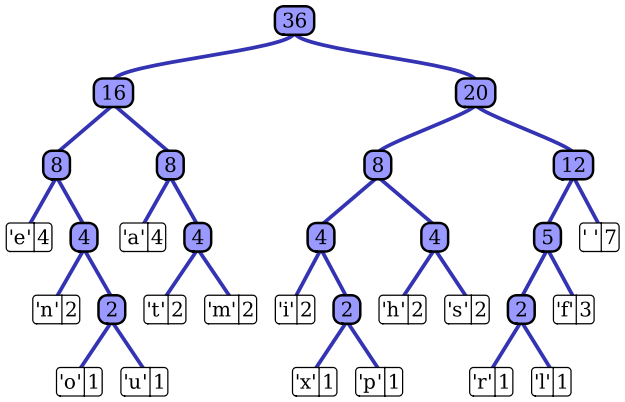
\includegraphics[width=1.0\textwidth]{Huffman}
    \caption{Ejemplo de un árbol de Huffman}
    \label{fig:huffman}
\end{figure}

Los códigos se generan a partir del camino que se toma para llegar al símbolo
en el árbol. $0$ para rama izquierda, $1$ para rama derecha. En este ejemplo, a
la letra `e' le corresponde el código \verb+000+ y a la letra `a' \verb+010+.
Para estas dos letras se está usando 3 ($37.5\%$) de los 8 bits que se
usan comúnmente para representar letras en inglés.

El estándar proporciona un código de Huffman de referencia para las
implementaciones. La implementación descrita aquí utiliza los códigos de
referencia.
% pero cuenta con la posibilidad de hacer un código diferente para cada
% imagen, al costo extra de tiempo de codificación y de complejidad de
% implementación.

La segunda opción que nos da la especificación es la \emph{\gls{codificación
aritmética}}. No es popular, ya que hay muchas patentes relacionadas a la
técnica, pero para compresión es un método superior.

Aunque los árboles de Huffman son óptimos para comprimir símbolos
separadamente, la codificación aritmética obtiene mejores resultados porque
codifica varios símbolos como coeficientes de polinomios. A cada símbolo le
corresponde un entero único relacionado a la frecuencia en la que ocurre en el
mensaje, y ese número se usa como el coeficiente. El grado del polinomio es la
longitud del mensaje.

\subsection{Resumen de la vida de un bloque}

Lo que se hace en JPEG es convertir la imagen a \verb+YUV+, partirla en bloques
de $8\times8$ para cada componente, aplicar DCT a cada bloque, cuantificar y,
finalmente, aplicar codificación de Huffman o aritmética. Los bloques se
escriben secuencialmente a disco en formato \verb+YUV YUV YUV (...)+. Este
trabajo se enfoca en usar heurísticas para encontrar tablas de cuantificación
de manera individual para cada imagen a codificar.

%%% Local Variables:
%%% mode: latex
%%% ispell-local-dictionary: "espanol"
%%% TeX-engine: xelatex
%%% TeX-master: "../tesis"
%
